\begin{Answer}{1}
	\begin{enumerate}[a),leftmargin=*]
		\i \hspace*{150pt}
		\begin{tikzpicture}
			\draw (-4,0) -- (4,0);
			\filldraw[black] (-2,0) circle[radius = 2pt] node[above] {$A$};
			\filldraw[black] (2,0) circle[radius = 2pt] node[above] {$B$};
		\end{tikzpicture}
		\i \hspace*{150pt}
		
\begin{tikzpicture}
			\draw (-4,0) -- (4,0);
			\filldraw[black] (-2,0) circle[radius = 2pt] node[above] {$A$};
			\filldraw[black] (0,0) circle[radius = 2pt] node[above] {$C$};
			\filldraw[black] (2,0) circle[radius = 2pt] node[above] {$B$};
		\end{tikzpicture}
		\i \hspace*{150pt}
		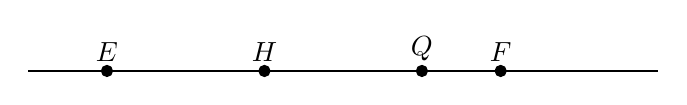
\begin{tikzpicture}
			\draw (-4,0) -- (4,0);
			\filldraw[black] (-3,0) circle[radius = 2pt] node[above] {$E$};
			\filldraw[black] (-1,0) circle[radius = 2pt] node[above] {$H$};
			\filldraw[black] (1,0) circle[radius = 2pt] node[above] {$Q$};
			\filldraw[black] (2,0) circle[radius = 2pt] node[above] {$F$};
		\end{tikzpicture}
		\i \hspace*{150pt}
		\begin{tikzpicture}
			
		\end{tikzpicture}
		\i \hspace*{150pt}
		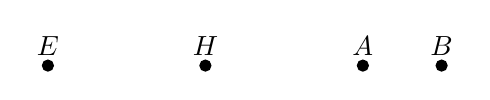
\begin{tikzpicture}
			\filldraw[black] (-3,0) circle[radius = 2pt] node[above] {$E$};
			\filldraw[black] (-1,0) circle[radius = 2pt] node[above] {$H$};
			\filldraw[black] (1,0) circle[radius = 2pt] node[above] {$A$};
			\filldraw[black] (2,0) circle[radius = 2pt] node[above] {$B$};
		\end{tikzpicture}
	\end{enumerate}
	
\end{Answer}
